\documentclass[]{fithesis3}
\usepackage[
	main=czech,
	english
]{babel}

\usepackage{enumitem}

\thesissetup{
    date          = \the\year/\the\month/\the\day,
    university    = mu,
    faculty       = fi,
    type          = bc,
    author        = Ondřej Přikryl,
    gender        = m,
    advisor       = {RNDr. Michal Procházka, Ph.D.},
    title         = {Integrace RemSig do klientských aplikací},
    keywords      = {Digitální podpis, RemSig, OAuth 2.0, PKCS\#11, CryptoAPI, CNG, CSP, Smart Card Minidriver},
}

\thesislong{abstract}{
Bakalářská práce se věnuje digitálnímu podpisu, popisuje vzdálené úložiště certifikátů a privátních klíčů RemSig a představuje moduly, které slouží k integraci jeho funkcí do klientských aplikací. V práci je popsán standard PKCS\#11 a kryptografické prostředí operačního systému Microsoft Windows. Jako autentizační metoda ke vzdálenému úložišti je použit protokol OAuth 2.0.
}
\thesislong{thanks}{
Rád bych poděkoval panu RNDr. Michalu Procházkovi, Ph.D. za cenné rady, věcné připomínky a vstřícnost při konzultacích a vypracování bakalářské práce.	
}

\begin{document}
\chapter{Úvod}

Prvky informačních technologií se stávají každodenní součástí života a většina lidí by si bez nich již nedokázala život představit. Informační technologie uživatelům v mnoha směrech usnadňují život. Slouží jak k práci, tak i ke komunikaci se známými, zábavě a mnoha dalším činnostem. S rozšířením se však zvyšuje i potenciální riziko, které zneužití těchto prvků přináší. V době, kdy internet poskytuje základní komunikaci mezi více než miliardou lidí a je čím dál tím více používán jako nástroj k obchodování, se bezpečnost stává nesmírně důležitou otázkou, která by neměla zůstat nepovšimnuta. Částečnou odpovědí na tuto otázku bylo zavedení kryptografických systémů. I ty však nenabízí řešení ve všech případech a lidé by si měli stále dávat velký pozor. 

Kryptografie nebyla původní součástí návrhu internetu, ale v posledních dekádách se díky rozmachu digitálních technologií stala důležitým prvkem internetové infrastruktury. Přestože je skryta před zraky laických uživatelů, jde o důležitý vědní obor, který v současnosti prožívá obrovský posun kupředu. Tento vývoj je způsoben zejména tím, že si uživatelé začínají uvědomovat potřebu chránit své data a soukromí i ve virtuálním světě. Moderní kryptografie má mnoho podob a odvětví, jednou z nich je digitální podpis (též nazýván elektronický podpis), který je nezbytnou součástí systému RemSig.

Systém RemSig je bezpečné vzdálené úložiště certifikátů a privátních klíčů, které uživatelům poskytuje možnost podepisovat dokumenty bez nutnosti neustálého fyzického přístupu k zařízení, na němž je certifikát uložen. Důležitou součástí systému RemSig je uživatelská přívětivost. V současné době je systém možné používat pouze z\,webového rozhraní INET
\footnote{Inet MU, viz. \url{https://inet.muni.cz}.} 
a IS MU
\footnote{Informační systém Masarykovy univerzity, viz. \url{https://is.muni.cz}.}
, a proto je nutná implementace knihoven, které integrují funkce RemSigu do klientských aplikací. Náplní mé bakalářské práce je tyto knihovny implementovat a popsat základní prvky CSP a PKCS\#11. 


Struktura bakalářské práce je následující. První kapitola je věnována úvodu. Druhá kapitola se věnuje základnímu principu digitálních podpisů. Následující kapitola obsahuje popis systému RemSig, jeho vlastnosti a funkcionalitu. Čtvrtá kapitola se zabývá protokolem OAuth 2.0, jeho využitím a schopnostmi. Pátá kapitola popisuje standard PKCS\#11. Šestá kapitola je poslední kapitolou teoretické části bakalářské práce a věnuje se CryptoAPI, pod kterou spadá většina kryptografie u operačních systémů Microsoft Windows. Sedmá kapitola se zabývá praktickou částí práce. Popisuje implementaci knihoven, úpravy systému RemSig a potřebnou implementaci virtuálního tokenu do budoucna. V osmé kapitole následuje shrnutí výsledků a\,závěr bakalářské práce.
%V první fázi práce se zaměřuji na vytvoření knihovny v programovacím jazyce C. Tato knihovna %obsahuje základní funkce pro práci s úložištěm certifikátů v operačním systému Windows pomocí %vývojového prostředí Cryptography API: Next Generation3 (dále CNG). V druhé fázi je zapotřebí %vytvořit knihovnu poskytující komunikaci mezi klientem a serverem a pomocí otevřeného %protokolu OAuth 2.0 získat přístup k datům uloženým na serveru RemSig. V poslední fázi spojuji již %implementované knihovny do fungujícího celku.

Očekávaným cílem bakalářské práce jsou knihovny propojující RemSig a klientské aplikace . Důsledkem toho již není zapotřebí používat webové rozhraní INET a IS MU, což zaměstnancům MU výrazně usnadní práci při podepisování digitálních dokumentů. 


\chapter{Digitální podpis}

Digitální podpis slouží k nahrazení obyčejného podpisu v digitálním světě. Je založen na asymetrické kryptografii a k jeho použití je zapotřebí dvojice klíčů - soukromého a veřejného. Digitální podpis zaručuje následující vlastnosti:
\begin{itemize}
\item Autenticitu - každý podpis je jednoznačně spojen s uživatelskou entitou, kterou může být jak běžný uživatel, tak i organizace nebo státní útvar (digitální značka).
\item Integritu dat - zaručuje, že data nebyla po cestě pozměněna. To je velice důležité k ujištění, že data, která byla odeslána, druhá strana také přijala.
\item Nepopiratelnost - autor nemůže popřít, že data nepodepsal. To je zajištěno tím, že k vytvoření podpisu je zapotřebí soukromý klíč, který má vlastník podpisu v držení a není veřejně znám.
\end{itemize} 
\section{Princip použití}
Uživatel si vytvoří dvojici klíčů, veřejný a soukromý. Soukromý klíč si ponechá a veřejný nechá potvrdit certifikační autoritou a následně jej zveřejní. Podepsaný veřejný klíč nazýváme certifikát. Podpis dokumentu poté probíhá následovně:
\begin{itemize}
\item uživatel spočítá haš (ang. hash) dokumentu - například pomocí rychlé hašovací funkce SHA256
\item haš zašifruje svým soukromým klíčem - například pomocí algoritmu RSA
\item data poté odešle společně s certifikátem a zašifrovaným hašem
\end{itemize}
Ověřování podpisu probíhá analogicky:
\begin{itemize}
\item osoba, provádějící ověření, spočítá haš dokumentu
\item za pomoci veřejného klíče osoby, která dokument podepsala, dešifruje přijatý digitální podpis a ověří, že získaný haš je shodný s vypočteným hašem
\end{itemize}
\begin{figure}[!ht]
  	\begin{minipage}{1.00\textwidth}
    		\includegraphics[width=\textwidth]{/home/oprikryl/Skola/bakalarka/obrazky/signature.png}
  	\end{minipage}
 	\caption{Principy digitálního podpisu.}
  	\label{fig:Digitální podpis.}
\end{figure}
Pokud si haše odpovídají, pak je jisté, že přijatý dokument je shodný s\,odeslaným a je tedy zaručena integrita. Aby byla zajištěna nepopiratelnost a autenticita, je nutné ověřit, že daný klíč opravdu patří osobě, která poslala podepsaný dokument. Procesu, který toto zajišťuje, se\,říká \textit{přenos důvěry}. 

\section{Přenos důvěry}
Aby bylo možné pomocí digitálního podpisu dosáhnout autenticity a\,nepopiratelnosti, je veřejný klíč dané osoby podepsán důvěryhodnou certifikační autoritou. Tímto způsobem je vyjádřeno, že certifikační autorita věří, že majitel veřejného klíče je skutečně ten, za koho se vydává. Uživatel musí certifikační autoritě prokázat svoji totožnost předtím, než získá certifikát.
Další možností k dosažení autenticity je tzv. \textit{síť důvěry}. Jedná se o decentralizovanou alternativu k centralizovanému modelu certifikačních autorit. [1]

\chapter{RemSig}

Systém RemSig je bezpečné vzdálené úložiště certifikátů a privátních klíčů, které uživatelům poskytuje možnost podepisovat dokumenty bez nutnosti neustálého fyzického přístupu k zařízení, na němž je certifikát uložen. Díky tomu odpadá uživatelům systému RemSig povinnost nosit s sebou hardwarové zařízení, což zvyšuje uživatelskou přívětivost i funkcionalitu. Uživatelé totiž mohou podepisovat dokumenty, i když u sebe právě nemají kryptografické zařízení, nebo když jsou na jiném počítači, který není nakonfigurovaný pro práci s\,digitálními podpisy nebo není důvěryhodný. [2]

	\section{Aktuální využití}

		RemSig umožňuje podepisování dokumentů přímo z webového rozhraní systému INET
		a IS MU a je v souladu se současnou českou legislativou. RemSig je napojen na služby 				certifikační autority PostSignum
	\footnote{Kvalifikovaná certifikační autorita České Republiky, viz. \url{www.postsignum.cz/}.}, 			což je další výhodou pro zaměstnance MU, kteří tak nemusí řešit vydání certifikátu třetí 			stranou, ale vše si pohodlně nastaví v\,rozhraní INET. Aktuálně je používána verze 					implementovaná v jazyce PHP, ale k dispozici je již nová verze implementovaná v jazyce 			Java, která již brzy nahradí starou implementaci. 
	
	\section{Autorizace} 

	Pro přístup k API systému je zapotřebí, aby se uživatel autentizoval klientovi, který 				zprostředkovává komunikaci mezi uživatelem a\,veřejně přístupnou API RemSigu.  
	\begin{figure}[!h]
  	\begin{minipage}{1.00\textwidth}
    		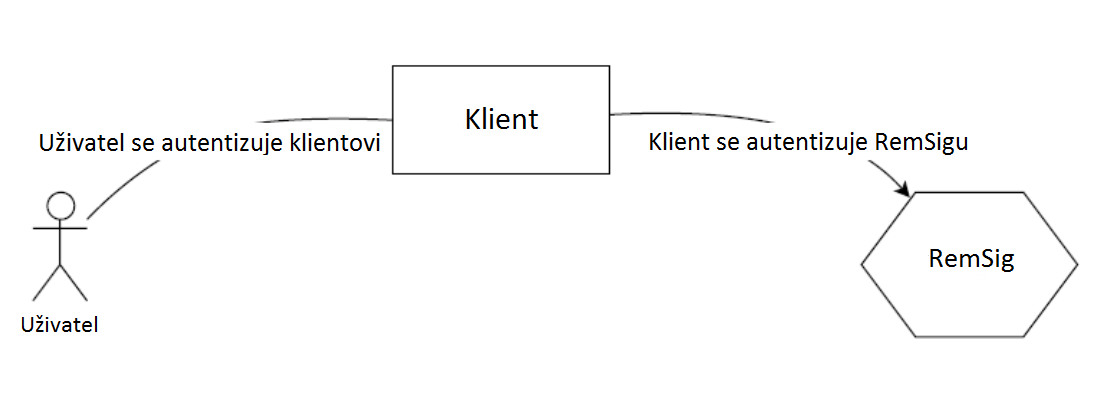
\includegraphics[width=\textwidth]{/home/oprikryl/Skola/bakalarka/obrazky/RemSigAten.png}
  	\end{minipage}
 	\caption{RemSig - Autentizace pomocí klienta.}
  	\label{fig:RemSig - Autentizace pomocí klienta.}
	\end{figure}
	Po autentizaci uživatele, Remsig obdrží od klienta unikátní identifikátor, podle kterého určí, ke 		kterým operacím je klient autorizován. Jestliže se identifikátor nenachází v\,seznamu pro řízení 		přístupu (ACL - Access Control List)
	\footnote{Více o ACL viz. \url{https://cs.wikipedia.org/wiki/Access_control_list}.} , klient není oprávněn k\,žádné operaci.

		\subsection{Autentizace certifikátem}

		V nové verzi je podporována autentizace certifikátem. Poté, co se uživatel autentizuje 				klientovi, klient odešle RemSigu certifikát, pomocí kterého RemSig určí, ke kterým 				operacím je klient oprávněn. Tento přístup však není vyhovující v případech, kdy chce 			klient komunikovat přímo s RemSigem. K tomu slouží protokol OpenID Connect.

		\subsection{OpenID Connect}

		OpenID Connect je již třetí verzí protokolu OpenID. Jedná se o protokol sloužící k 					ověřování identit, který staví na protokolu OAuth 2.0.  OpenID Connect umožňuje 				klientovi ověřit identitu koncového uživatele a získat základní informace o profilu. 					Podrobnému popisu protokolu OAuth 2.0 je věnována vlastní kapitola.

	\section{Role} 	
	Po úspěšné autentizaci získá klient přístup k metodám odpovídajícím jeho roli. RemSig rozlišuje 		dva typy rolí:
	\begin{itemize}
		\item Signer - podepisující
		\item Manager - manažer
	\end{itemize}
	\newpage
	Uživatelé systému IS MU mají roli podepisujícího. Ten má přístup k následujícím operacím:
	\begin{itemize}
		\item \textit{sign} - podepíše data podle defaultních kryptografických mechanismů
		\item \textit{signPKCS7} - vytvoří PKCS\#7
			\footnote{Více o standardu PKCS\#7 na \url{http://www.emc.com/emc-plus/rsa-labs/standards-initiatives/pkcs-7-cryptographic-message-syntax-standar.htm}.} podpis dat
		\item \textit{signPdf} - slouží k podepisování PDF dokumentů
	\end{itemize}
	Zatímco manažer má přístup k následujícím operacím:
	\begin{itemize}
		\item \textit{importCertificate} - importuje certifikát do systému RemSig
		\item \textit{importPKCS12} - importuje strukturu dle standardu PKCS\#12
		\footnote{Více na \url{http://www.emc.com/emc-plus/rsa-labs/standards-initiatives/pkcs12-personal-information-exchange-syntax-standard.htm}.}
		\item \textit{exportPKCS12} - exportuje soukromý klíč a certifikát ve struktuře 					definované standardem PKCS\#12
		\item \textit{changePassword} - změní heslo, kterým je chráněn soukromý klíč
		\item \textit{changeCertificateStatus} - změní status certifikátu
		\item \textit{listCertificates} - vypíše všechny certifikáty uložené v systému RemSig
		\item \textit{checkPassword} - zjistí, zda-li poskytnuté heslo skutečně slouží pro 					odemknutí soukromého klíče
	\end{itemize}

	\section{Funkcionalita}
	Volání metod probíhá pomocí veřejně dostupné API. Při požadavku se klient musí autentizovat 		pomocí přístupového tokenu nebo certifikátu. Parametry a data jsou posílány formou XML 			dokumentu pomocí metody HTTP POST. Data odeslána RemSigu na podpis musí být 				kódována metodou BASE64\footnote{Více o kódování BASE64 na \url{https://cs.wikipedia.org/wiki/Base64}.}, přijatá 		data jsou také kódována pomocí BASE64. Kvůli 	bezpečnosti je použit protokol HTTPS.

		\begin{figure}[!ht]
  			\begin{minipage}{1.00\textwidth}
    			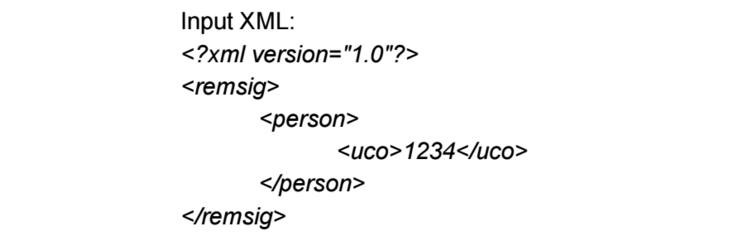
\includegraphics[width=\textwidth]{/home/oprikryl/Skola/bakalarka/obrazky/xml_input.png}
  			\end{minipage}
 			\caption{Ukázka XML požadavku metody \textit{listCertificates}.}
  			\label{fig:Ukázka XML požadavku.}
		\end{figure}

		\begin{figure}[!ht]
  			\begin{minipage}{1.00\textwidth}
    			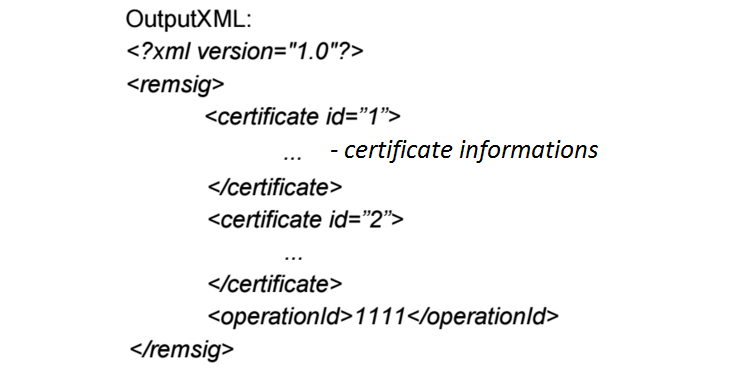
\includegraphics[width=\textwidth]{/home/oprikryl/Skola/bakalarka/obrazky/xml_output.png}
  			\end{minipage}
 			\caption{Ukázka XML odpovědi metody \textit{listCertificates}.}
  			\label{fig:Ukázka XML odpovědi.}
		\end{figure}

	\subsection{Správa úložiště}
	
	Aby uživatel mohl používat systém RemSig, musí v něm mít uložen certifikát a soukromý klíč. 		Remsig umožňuje generování dvojice soukromého a veřejného klíče přímo v systému. Po 			vygenerování je soukromý klíč zašifrován pomocí přiloženého PINu, který si uživatel sám zvolí. 		Dvojice je poté uložena do úložiště a klientovi je nazpět zaslán veřejný klíč, který je potřeba 		podepsat certifikační autoritou. Podepsaný certifikát je nutno opět odeslat systému. Uživatel 		však nemusí použít systém pro generování nové dvojice, ale může importovat již existující 			dvojici ve struktuře PKCS\#12 do systému.

	\begin{itemize}
	\item Import certifikátu 

		Metoda \textit{importCertificate} slouží k importování certifikátu do úložiště. Certifikát 			musí být ve formátu PEM. Tato metoda je používána v případě, kdy byla dvojice klíčů 				vygenerována systémem RemSig a veřejný klíč byl předán na podepsání certifikační 				autoritou.

	\item Import struktury PKCS\#12

		Metoda \textit{importPKCS12} slouží k nahrání dvojice vytvořené mimo systém RemSig. 			Tato dvojice je uložena ve struktuře PKCS\#12, která je zabezpečena heslem. Poté, co 			uživatel zadá heslo, je ze struktury exportována dvojice a uložena do úložiště RemSig. 				Uživatel musí poskytnout nové heslo, kterým bude zašifrován soukromý klíč.

	\item Export struktury PKCS\#12

		Metoda \textit{exportPKCS12} slouží k exportování dvojice ze systému RemSig. Jedinou 			možností jak exportovat certifikát a soukromý klíč je vytvořením PKCS\#12 struktury, do 		které je po zadání uživatelova PINu k soukromému klíči uložen certifikát a dešifrovaný 				soukromý klíč. Celá struktura je posléze zamknuta heslem.
	\end{itemize}

	\subsection{Podepisování dat}

	Jestliže má uživatel k dispozici certifikát a soukromý klíč, může začít používat metody 				vzdáleného podpisu. RemSig má k dispozici tři metody na podepisování dat.

	\begin{itemize}
	\item Defaultní podpis
		
		Metoda \textit{sign} slouží k podpisu dat. K podpisu je použit defaultní kryptografický 				mechanismus. 
	
	\item PKCS\#7 podpis

		Digitální podpisy se od sebe mohou lišit v použitých algoritmech, ve formátu výstupu a v 			tom, zda-li výsledný podpis má být přiložen k datům či má být obdržen samostatně. 		

		Metoda \textit{signPKCS7} umožňuje nastavit tyto hodnoty a vytvořit podpis dle 					standardu PKCS\#7. Systém RemSig používá k nastavení těchto hodnot tzv. 						\textit{prifily}.

		Profily \newline
		Jestliže má organizace specifické požadavky na PKCS\#7 podpis, může si vytvořit profil, ve 		kterém si nastaví požadované hodnoty. Při vytváření nového profilu musí být nastaveny 			následující atributy:

		\begin{itemize}
		\item algorithm - algoritmus, který bude použit k podpisu
		\item no-detach - určuje, zda-li bude podpis přiložen k datům
		\item encoding - určuje formát výstupu
		\end{itemize}

		\begin{figure}[!h]
  			\begin{minipage}{1.00\textwidth}
    			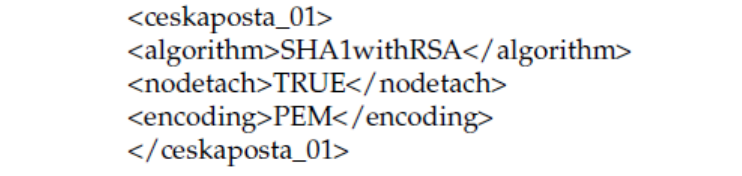
\includegraphics[width=\textwidth]{/home/oprikryl/Skola/bakalarka/obrazky/profile_ceskaposta.png}
  			\end{minipage}
 			\caption{Profil české pošty.}
  			\label{fig:Profil české pošty.}
		\end{figure}

		Na obrázku je uveden profil české pošty s označením jedna. Metoda s tímto profilem 				použije k vytvoření haše dat algoritmus SHA1 a výsledný haš zašifruje pomocí algoritmu 			RSA, podpis bude přiložen společně s daty a výstup bude ve formátu PEM.

	\item Podpis PDF dokumentu

	Pro podepisování PDF dokumentů slouží metoda \textit{signPdf}. Uživatel si zde může zvolit, 		zda bude vložen vodoznak do dokumentu či ne. K dispozici je již přednastavený vodoznak pro 		dokumenty MU. Uživatel si však může vytvořit vlastní nastavení, ve kterém je možné uvést 		pozici vodoznaku, stránky na kterých bude vodoznak umístěn, obrázek pozadí vodoznaku a 			text, který bude obsahovat.
	\end{itemize}	

\chapter{OAuth 2.0}

OAuth 2.0 (RFC 6749) je autorizační protokol (resp. framework), který umožňuje aplikacím třetích stran získat přístup ke službám HTTP, a\,to buď jménem registrovaného uživatele anebo jménem aplikace třetí strany. Protokol specifikuje pouze autentizaci klienta a výdej přístupového tokenu, přístup k jednotlivým zdrojům je již zcela nezávislý na protokolu. Je tedy zapotřebí veřejně dostupné API. Protokol OAuth 2.0 nahrazuje starý protokol OAuth 1.0 a není s ním zpětně kompatibilní.

	\section{Motivace}

	V tradičním modelu autentizace klient-server, žádá-li uživatel o přístup k zabezpečenému 			obsahu, je zapotřebí jeho autentizace pomocí přihlašovacích údajů. Aby tedy aplikace třetí 			strany mohla přistoupit k témuž obsahu, je zapotřebí s ní sdílet přihlašovací údaje oprávněné 		osoby. To však s sebou přináší několik problémů:

		\begin{itemize}
  		\item 
		Aplikace třetích stran si uchovávají přihlašovací údaje k budoucímu použití. Údaje bývají 			většinou uchovávány v otevřené podobě. Uchovávání pouze otisku je nedostatečné.

 		 \item 
		Uživatel ve většině případů nemůže omezit přístup aplikace k\,chráněnému obsahu, a to 			jak časovou platností, tak i omezením obsahu, ke kterému získá aplikace přístup.

 		 \item 
		Obvykle lze odebrat přístup aplikaci k zabezpečenému obsahu pouze 							změnou hesla. To se však projeví i u dalších aplikací, které jsou závislé na stejných 				přihlašovacích údajích.

  		\item 
		Kompromitace aplikace třetí strany znamená ohrožení přihlašovacích údajů 						uživatele a všech souborů na nich závislých.
		\end{itemize}

	OAuth tyto problémy řeší zavedením autorizační vrstvy a oddělením rolí klienta 					(aplikace) a vlastníka chráněného zdroje. V protokolu aplikace zažádá o přístup ke 				chráněnému obsahu  a jsou jí přiděleny přihlašovací údaje (přístupový token) odlišné od 			přihlašovacích údajů uživatele. [3]

	\section{Role}
		OAuth 2.0 definuje 4 typy rolí:

		\begin{itemize}
 		\item Vlastník zdrojů:
  		\newline
		Entita schopná přidělit přístup ke chráněnému obsahu. Jedná-li se o osobu, nazýváme ji 			koncový uživatel.
  		\item Server zdrojů:
  		\newline
		Poskytovatel a hostitel chráněného zdroje, schopný obsluhovat požadavky ke 					chráněnému zdroji pomocí přístupového tokenu.
 	 	\item Klient:
  		\newline
		Aplikace, která vyžaduje přístup ke chráněnému obsahu.
  		\item Autorizační server:
 		\newline
		Server, který vydává klientovi přístupový token po úspěšné autentizaci oprávněné osoby.
		\end{itemize}
		Protokol nijak nespecifikuje interakci mezi autorizačním serverem a\,serverem zdrojů. 				Může se jednat o nezávislé entity, ale i o jeden server. [4]

	\section{Přístupový token}	

	Pokaždé když klient potřebuje přistoupit k chráněnému obsahu, potřebuje přístupový token 			(anglicky \textit{access token}). Přístupový token je řetězec znaků, který opravňuje klienta k 		přístupu k chráněnému obsahu. V řetězci jsou skrytě uloženy informace o délce platnosti 			tokenu, o rozsahu přístupu k chráněnému obsahu a informace o vlastníkovi obsahu. Délka 			platnosti se může lišit implementací, ale typicky bývá platnost tokenu nastavena na 1 hodinu 		(3600 sekund).

	\section{Obnovující token}	

	Obnovující token (anglicky \textit{refresh token}) může být získán společně s\,přístupovým 			tokenem a slouží k obnovení přístupového tokenu po vypršení jeho platnosti. Možnost získání 		přístupového tokenu pomocí obnovujícího tokenu bývá ve většině případech omezena počtem. 

	\section{Průběh protokolu}

	OAuth definuje několik základních způsobů autentizace vedoucích k\,získání přístupového 			tokenu. Patří mezi ně:

		\begin{itemize}
 		\item Autorizačním kódem:
  		\newline
		Jedná se o doporučený průběh, ke kterému je zapotřebí internetový prohlížeč. Klient s použitím prohlížeče přesměruje uživatele na přihlašovací stránku. Po 			úspěšné autentizaci zašle autorizační server klientovi autorizační kód. Klient pro získání 			přístupového tokenu zašle autorizační kód autorizačnímu serveru.
  		\item Implicitně:
  		\newline
		Tento typ je zjednodušením průběhu autorizace autorizačním kódem. Slouží pro aplikace 			běžící v prohlížeči, které používají skriptovací jazyky jako je například JavaScript. Na rozdíl 		od předchozího typu, klient získá přístupový token přímo po přihlášení. Tento typ je 				rychlejší,	jelikož redukuje počet výzev a\,odpovědí, které je potřeba udělat pro získání 				tokenu.
 	 	\item Zasláním přihlašovacích údajů:
  		\newline
		V tomto typu uživatel poskytne přihlašovací údaje klientovi. Klient zašle přihlašovací údaje 		autorizačnímu serveru, který po úspěšné autentizaci uživatele zašle zpět přístupový 				token. Přihlašovací údaje jsou použity jen pro získání přístupového a\,obnovujícího tokenu, 			není tedy potřeba jejich uložení pro budoucí použití. Tento typ je používán pouze při 				vysoké důvěře mezi uživatelem a aplikací. 
		\end{itemize}
		
	\newpage

	\section{Registrace klienta}

	Předtím než začne klient používat protokol, je potřeba jeho registrace na autorizačním serveru. 	Pro zvýšení bezpečnosti by klient měl poskytnout:

	\begin{itemize}
  		\item jeho typ - webová aplikace, nativní aplikace, zařízení
		\item adresu, na kterou bude token přesměrován
		\item jakoukoliv jinou informaci, kterou autorizační server požaduje (název, popis, smluvní 				podmínky, atd...).
	\end{itemize}

	Poté co se klient úspěšně zaregistruje, obdrží od autorizačního serveru unikátní identifikátor a 		heslo. Tyto údaje jsou nutné pro autentizaci klienta serveru během průběhu protokolu. Je-li při 		průběhu vyžadována adresa přesměrování, tak musí souhlasit s adresou uvedenou klientem při 	registraci.

	\begin{figure}[!ht]
  		\begin{minipage}{1.00\textwidth}
    			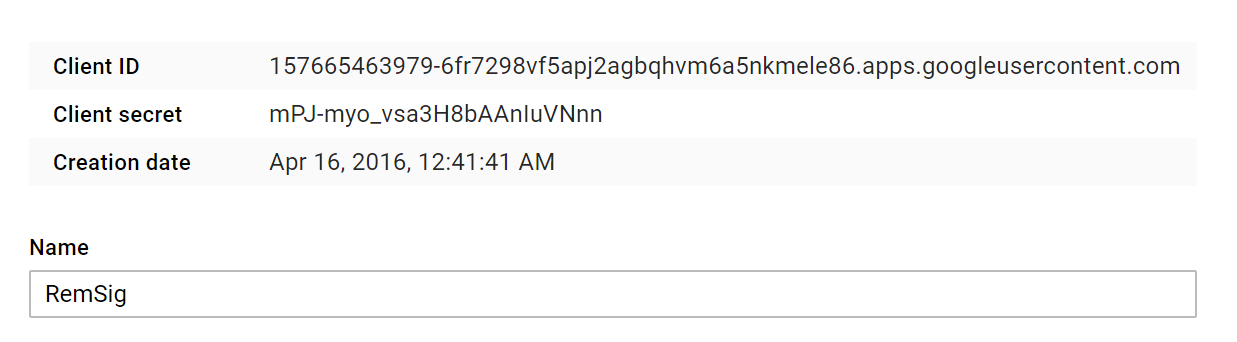
\includegraphics[width=\textwidth]{/home/oprikryl/Skola/bakalarka/obrazky/RemSigRegistration.png}
  		\end{minipage}
 		\caption{Google OAuth - registrace klienta.}
  		\label{fig:Google OAuth - registrace klienta.}
	\end{figure}	
	\newpage

\chapter{PKCS\#11}

S nástupem kryptografie přišla nutnost zavést jednotné protokoly a\,postupy pro zajištění kompatibility koncových aplikací. Ačkoliv se vývojáři shodli na základních kryptografických postupech, kompatibilita mezi jednotlivými implementacemi nebyla nikdy zaručena. Jednotný standard byl tedy nutností. Tuto potřebu naplnila organizace RSA Laboritories zavedením jednotného standardu Public-Key Cryptography Standards, zkráceně PKCS. Jedná se o celou rodinu standardů, mezi které patří například i PKCS\#11, který je využit v\,implementaci knihoven RemSig.

PKCS\#11 je platformově nezávislé aplikační programové rozhraní (API) pro kryptografické tokeny, nazývané Cryptoki podle Cryptographic Token Interface. PKCS\#11 je nyní ve verzi 2.20 a to již od roku 2004. S ohledem na stáří protokolu probíhá od roku 2009 testování nové verze protokolu s označením 2.30, který však ještě nebyl standardizován. [5]

	\section{Cíle návrhu}

	Cryptoki byl navržen s důrazem na jednotnost přístupu k rozdílným zařízením. Cílem rozhraní je 		poskytnout vyšší aplikační vrstvě shodný přístup ke kryptografickému zařízení bez ohledu na 		konkrétní typ zařízení. Může se tak jednat o 
	Smart Card \footnote{Více o Smart Card na \url{https://cs.wikipedia.org/wiki/Smart_Card}.} 
	, 
	PCMCIA \footnote{Více o PCMCIA na \url{https://cs.wikipedia.org/wiki/PCMCIA}.} 
	kartu nebo síťovou službu, aplikace využívající Cryptoki s nimi může pracovat bez ohledu na 		jejich hardwarovou odlišnost.

	Druhotným cílem bylo sdílení prostředků. S rozvojem víceúlohových operačních systémů se 		stalo žádoucím být schopen sdílet jedno zařízení mezi více aplikacemi. Stejně tak jedna 			aplikace by měla být schopna operovat s více kryptografickými zařízeními.

	\section{Model návrhu}

	Model použití Cryptoki začíná jednou nebo více aplikacemi, které požadují přístup k jednomu 		nebo více kryptografických zařízením. Tyto zařízení provedou operace požadované aplikací a 		vrátí výsledek.
	\begin{figure}[!ht]
  		\begin{minipage}{1.00\textwidth}
    			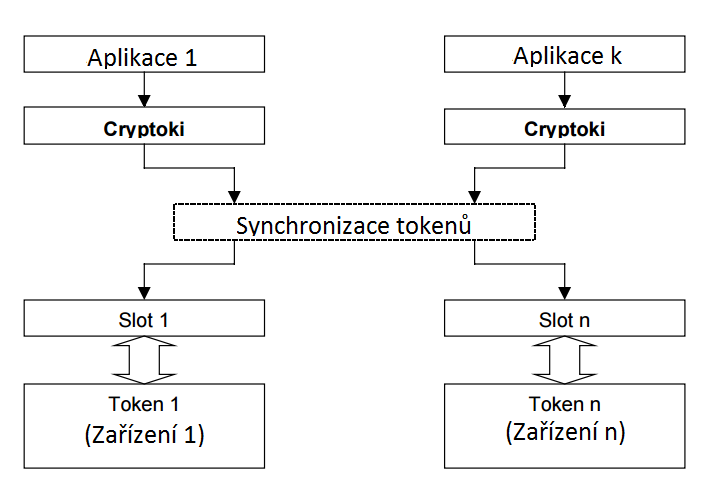
\includegraphics[width=\textwidth]{/home/oprikryl/Skola/bakalarka/obrazky/pkcs11_general_model.png}
  		\end{minipage}
 		\caption{PKCS11 - Obecný model.}
  		\label{fig:PKCS11 - Obecný model.}
	\end{figure}

	Cryptoki je tedy rozhraní mezi vyšší vrstvou uživatelských aplikací a nižší hardwarovou 			vrstvou, která vykonává kryptografické operace. Jak bylo popsáno výše, tato hardwarová 			vrstva může být reprezentována kartami, tokeny nebo dokonce vzdálenými síťovými službami.

	Díky tomu, že Cryptoki maskuje skutečnou hardwarovou podobu připojeného zařízení a 			zobrazuje je jako totožné jednotky, volající aplikace nemusí znát přesné rozhraní, ke kterému je 		zařízení připojeno, či jaký ovladač pro ně použít.

	Je nutné podotknout, že Cryptoki nepředpisuje, aby všechny jeho funkce byli implementovány. 		Standard však definuje, které funkce implementovány být musí, aby modul poskytoval nějakou 		funkcionalitu. Díky této vlastnosti se začali objevovat tzv. \textit{profily} PKCS\#11. [7]

		\subsection{Objekty}

		Cryptoki vidí token jako zařízení, na kterém jsou uchovávány objekty a\,které může vykonávat 			kryptografické operace. Cryptoki definuje tři základní typy objektů:
		\begin{itemize}
			\item data - jsou definovány a spravovány aplikacemi
			\item certifikáty - uchovává certifikáty veřejného klíče
			\item klíče - uchovává kryptografické klíče
		\end{itemize}

		\begin{figure}[!ht]
  			\begin{minipage}{1.00\textwidth}
    				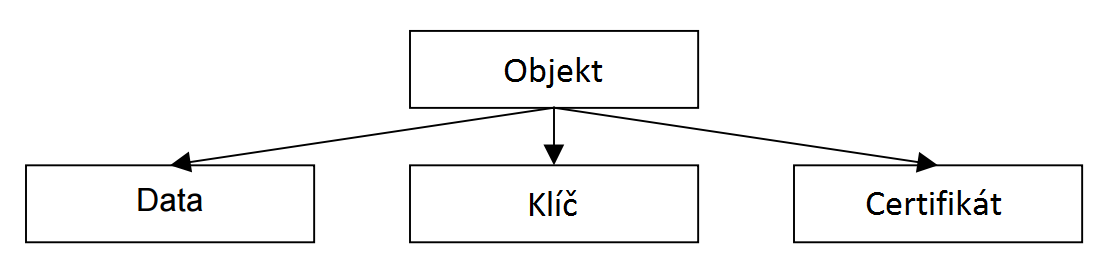
\includegraphics[width=\textwidth]{/home/oprikryl/Skola/bakalarka/obrazky/pkcs11_objekt.png}
  			\end{minipage}
 			\caption{PKCS11 - Objekty.}
  			\label{fig:PKCS11 - Objekty.}
		\end{figure}

		Objekty jsou zároveň klasifikovány dle jejich životnosti a viditelnosti. Do této skupiny patří 			\textit{session} a \textit{token} objekty. \textit{Token objekty} jsou objekty viditelné všem 			aplikacím připojeným k tokenu a jejich životnost není ovlivněna žádnou relací (tzn. 					setrvávají na tokenu, dokud nejsou odstraněny). Zatímco \textit{session objekty} jsou 				viditelné pouze aplikaci, která je vytvořila a zanikají s ukončením relace.
		Objekty se dále mohou dělit na soukromé a veřejné. Pro přístup k veřejnému objektu se 			aplikace nemusí autentizovat tokenu, zatímco u soukromých je požadováno přihlášení 				pomocí PINu nebo jiné autentizační metody (např. biometrická zařízení).

		\newpage
		\subsection{Uživatelé}

		Cryptoki definuje dva typy uživatelů: 
		\begin{itemize}
			\item Security Officer (dále již jen SO) 
			\item normální uživatel
		\end{itemize}
		Oba vykonávají v systému různé úlohy, ale standard nedefinuje jejich vzájemný vztah. Je 			tedy v pořádku, když je stejná osoba normálním uživatelem i SO.

		Účelem SO je inicializovat token a nastavit normálnímu uživateli PIN nebo jinou formu 				autentizace. SO, na rozdíl od normálního uživatele, dokáže přistoupit pouze k veřejným 			objektům.
		Normální uživatel je jediný, kdo může přistupovat k soukromým objektům, ale až poté co	
		se úspěšně autentizuje. 

		\subsection{Relace}

		Pro práci s funkcemi a objekty tokenu je potřeba vytvořit alespoň jednu relaci (ang. 				\textit{session}). Jedná se o logické spojení, ve kterém aplikace komunikuje s tokenem. 			Relace se dělí na dva základní druhy:
		\begin{itemize}
			\item R/O relace (pouze pro čtení) 
			\item R/W relace (pro čtení i zápis).
		\end{itemize}

		R/W relace umožňují aplikaci číst, vytvářet, modifikovat a mazat objekty uložené na 				tokenu, zatímco R/O relace má přístup pouze ke čtení těchto objektů. Toto omezení se 				však vztahuje pouze na \textit{token objekty}, nikoliv na \textit{session objekty}, ke 				kterým mají oba dva typy plný přístup. Po vytvoření relace má aplikace přístup pouze k 			veřejným objektům. Aby relace poskytovala přístup k soukromým objektům tokenu, je 				nutné, aby se uživatel autentizoval tokenu. 

		Cryptoki umožňuje aplikacím vytvářet k jednomu tokenu více relací, ale zároveň také 				umožňuje tokenu omezit počet R/O a R/W relací, které může aplikace využít. Při zániku 			relace jsou odstraněny všechny \textit{session objekty} této relace a to i v případě, že 				jsou tyto objekty používány jinou relací.

		\newpage
		\noindent Stavy
		\newline
		Otevřená relace může být v jednom z pěti možných stavů. Tyto stavy definují, které 				objekty budou dostupné a jaké operace na nich budou povoleny. Pro R/O relace platí:

		\begin{itemize}
			\item R/O Public Session

			Aplikace si otevřela R/O relaci a doposud není autentizována tokenu. Aplikace má 					právo ke čtení veřejných \textit{token objektů} a\,právo ke čtení/zápisu veřejných 					\textit{session objektů}.
	
			\item R/O User Functions

			Aplikace si otevřela R/O relaci a uživatel se autentizoval tokenu. Aplikace má přístup 				ke čtení všech \textit{token objektů} a právo ke čtení/zápisu všech \textit{session 				objektů}.
		\end{itemize}

		\begin{figure}[!ht]
  			\begin{minipage}{1.00\textwidth}
    				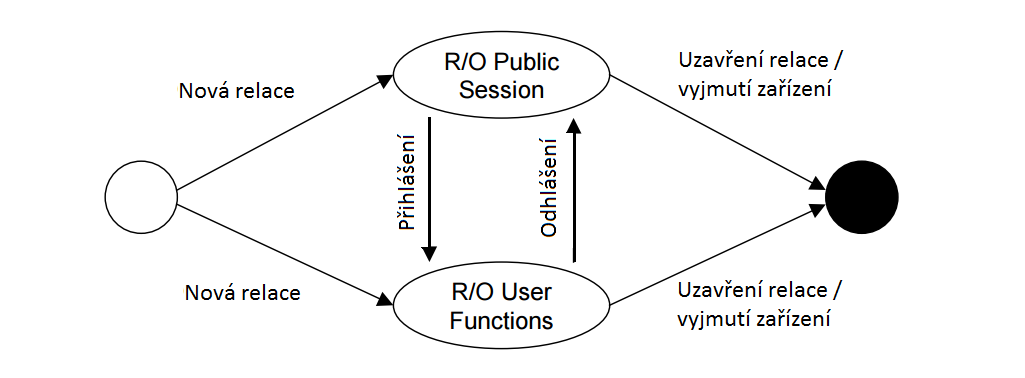
\includegraphics[width=\textwidth]{/home/oprikryl/Skola/bakalarka/obrazky/ro_sessions.png}
  			\end{minipage}
 			\caption{PKCS11 - Stavy R/O relací.}
  			\label{fig:PKCS11 - Stavy R/O relací.}
		\end{figure}

		\begin{itemize}
			\item R/W Public Session

			Aplikace si otevřela R/W relaci a doposud není autentizována tokenu. Aplikace má 				právo ke čtení/zápisu všech veřejných objektů.
	
			\item R/W User Functions

			Aplikace si otevřela R/W relaci a uživatel se autentizoval tokenu. Aplikace má přístup 			ke čtení/zápisu všech objektů.

			\item R/W SO Functions

			Aplikace si otevřela R/W relaci a SO se autentizoval tokenu. Aplikace má přístup 					pouze ke čtení/zápisu všech veřejných \textit{token objektů}. SO může nastavit PIN 				uživateli.
		\end{itemize}

		\begin{figure}[!ht]
  			\begin{minipage}{1.00\textwidth}
    				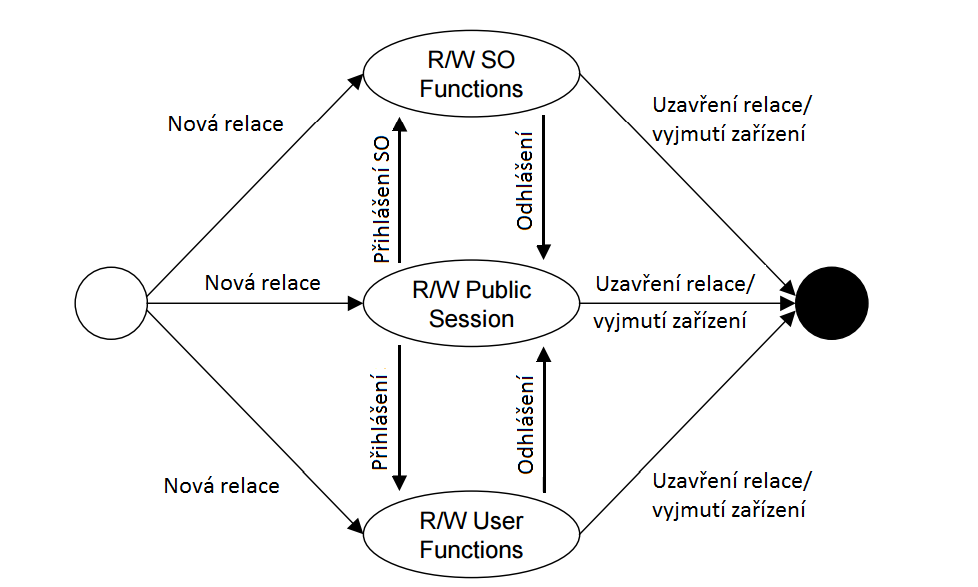
\includegraphics[width=\textwidth]{/home/oprikryl/Skola/bakalarka/obrazky/rw_sessions.png}
  			\end{minipage}
 			\caption{PKCS11 - Stavy R/W relací.}
  			\label{fig:PKCS11 - Stavy R/W relací.}
		\end{figure}	
		
\chapter{CryptoAPI}

Microsoft CryptoAPI je aplikační programové rozhraní (též nazývané CAPI) dostupné v operačních systémech Microsoft Windows. Jedná se o skupinu knihoven, které implementují kryptografické mechanismy. CryptoAPI se poprvé objevilo v operačním systému Windows NT 4.0 a v dalších verzích OS bylo postupně zdokonalováno. API podporuje jak symetrickou, tak i asymetrickou kryptografii a poskytuje řadu užitečných kryptografických funkcí jako například kryptograficky bezpečný generátor pseudonáhodných čísel. [9]

S operačním systémem Windows Vista však přišel nový model s\,názvem Cryptography API: Next Generation (zkráceně CNG). Předpokládá se, že tento model v dlouhodobém časovém horizontu nahradí CryptoAPI. CNG rozšiřuje původní implementaci o nové algoritmy a\,funkce. V\,novém modelu přibyla kryptografie využívající eliptických křivek, která nabízí stejnou úroveň zabezpečení při použití kratšího klíče, což ji činí efektivnější než algoritmus RSA. V\,modelu přibyli také knihovna BaseCSP a Smart Card Minidriver, které usnadňují výrobcům čipových karet integraci funkcionality jejich karet do operačního systému Windows. [10]

	\section{CSP}
	
	Výrobci mohou použít funkcionalitu kryptografických rozhraní implementováním speciálního 			modulu. Tyto moduly se nazývají Cryptographic Service Providers (zkráceně CSP). Jedná se o 		knihovny, které jsou určeny k práci s kryptografickými funkcemi. CSP může 				implementovat veškerou funkcionalitu definovanou kryptografickými rozhraními od symetrické 		kryptografie po práci s klíči a úložištěm certifikátů systému Windows. [11]

	\section{BaseCSP}
	S příchodem nového kryptografického modelu Cryptography API: Next Generation přibyla také 		nová knihovna s názvem BaseCSP. Tato knihovna usnadňuje výrobcům čipových karet integraci 		funkcionality jejich karet do operačního systému Windows. Tím pádem již není potřeba budovat 		celé řešení skrze CSP, ale implementovat pouze menší část pomocí \textit{Smart Card 			Minidriveru}. Samotné BaseCSP poskytuje minidriveru rozsáhlou funkcionalitu, stará se o práci s 		certifikáty v úložišti certifikátů operačního systému Windows (anglicky označován jako 				\textit{CertStore}), umožňuje hašování dat pomocí mnoha dostupných hašovacích algoritmů a 		další. [12]

	\section{CNG KSP}
	Na rozdíl od CryptoAPI, Cryptography API: Next Generation rozděluje CSP na 2 základní prvky a 	to:
	\begin{itemize}
	\item Key Storage Provider (zkráceně KSP)
	\item Cryptographic Algorithm Provider (zkráceně CAP)
	\end{itemize}
	KSP je používán pro veškerou práci s úložištěm klíčů, zároveň však obsahuje i základní 				algoritmy pro hašování a podepisování dat.

	\section{Smart Card Minidriver}
	Smart Card Minidriver představuje alternativní cestu budování kryptografického modulu na rozdíl od implementace celého CSP. Jelikož používá funkce již dostupných BaseCSP nebo KSP, jeho 			implementace je velmi jednodušší a efektivnější. BaseCSP/KSP se stará o veškeré dění v rámci 		úložiště certifikátů, nabízí mnoho hašovacích funkcí a\,další.  \newline

	Minidriver je dostupný od operačního systému Windows Vista. V průběhu vývoje minidriveru byla		přidávána nová funkcionalita, knihovna má nyní verzi 7.07, s posledními aktualizacemi k datu 		25. února 2016. Starší nebo neaktualizované operační systémy mohou mít nižší verzi, avšak 		pro splnění základní funkcionality musí být podporována alespoň verze 4. \newline

	Na následujícím obrázku je uveden obecný model celého systému. Minidriver je zobrazen jako 		jedna ze tří alternativ implementace modulu pro práci s kryptografickými zařízeními.  [13]

		\begin{figure}[!ht]
  			\begin{minipage}{1.00\textwidth}
    				\includegraphics[width=\textwidth]{/home/oprikryl/Skola/bakalarka/obrazky/minidriver_tree.png}
  			\end{minipage}
 			\caption{Role minidriveru v systému.}
  			\label{fig:Role minidriveru v systému.}
		\end{figure}	

		\subsection{Role}
		
		Specifikace minidriveru definuje 3 základní typy rolí:
		\begin{itemize}
			\item admin
			\item uživatel
			\item kdokoliv
		\end{itemize}
		Úlohou administrátora je správa karty. Admin je jediný, kdo může inicializovat a smazat 				souborový systém. Dále může odblokovat PIN uživatele a jako jediný může nastavit 				kartě stav "pouze pro čtení". Role uživatele slouží pro práci s certifikáty a klíči, jako je 				vytváření, upravování a mazání kontejnerů a digitální podpis dat. Nepřihlášená entita má 			přístup pouze ke čtení veřejných souborů karty.

		\subsection{Kontejnery}
		CryptoApi a CNG používají pro ukládání klíčů takzvané \textit{kontejnery}. Model definuje 			2 typy asymetrických klíčů:
		\begin{itemize}
			\item Signature Only (klíč určený k digitálnímu podpisu dat)
			\item  Key Exchange (sloužící k výměně klíčů)
		\end{itemize}		
		Do každého kontejneru může být uložen maximálně jeden klíč od každého typu. Jestliže je 			do kontejneru přidán klíč stejného typu, původní klíč je přemazán.

		\subsection{File system}
		Každé zařízení, které použije minidriver musí mít specifický souborový systém. V případě, že 		karta používá jiný systém práce s daty, musí soubory emulovat.

		\begin{figure}[!ht]
  			\begin{minipage}{1.00\textwidth}
    				\includegraphics[width=\textwidth]{/home/oprikryl/Skola/bakalarka/obrazky/minidriver_file_system.png}
  			\end{minipage}
 			\caption{Souborový systém minidriveru.}
  			\label{fig:Souborový systém minidriveru.}
		\end{figure}	

		\begin{itemize}
			\item /cardid - soubor obsahuje 16 bytový identifikátor karty.
			\item /cardcf - uchovává cache karty. Kdykoliv je na kartě něco změněno, hodnota v 				souboru se zvýší, čímž je indikováno, že si systém musí znovu načíst všechny soubory.
			\item /cardapps - obsahuje 8 bytový název aplikační podsložky, pro CryptoAPI je název 			složky "mscp".
			\item /mscp/cmapfile - tento soubor obsahuje informace o kontejnerech, které jsou na 				kartě k dispozici.
			\item /mscp/ksc00 - soubor s digitálním certifikátem ve formátu DER.
			\item /mscp/msroots - obsahuje strom certifikačních autorit.
		\end{itemize}

		\subsection{Práce s registry}
		
		Pro každé kryptografické zařízení, které má být spuštěno pod minidriverem se musí 				vytvořit sada záznamů v registru. Záznamy jsou přidány do HKEY\_LOCAL\_MACHINE$\backslash$SOFTWARE$\backslash$Microsoft$\backslash$Crypto- graphy$\backslash$Calais$\backslash$SmartCards$\backslash$NázevVýrobce

		\begin{figure}[!ht]
  			\begin{minipage}{1.00\textwidth}
    				\includegraphics[width=\textwidth]{/home/oprikryl/Skola/bakalarka/obrazky/minidriver_registry.png}
  			\end{minipage}
 			\caption{Registrační soubor minidriveru.}
  			\label{fig:Registrační soubor minidriveru.}
		\end{figure}	

		Atribut ATR slouží v tomto kontextu k identifikaci karty, zatímco atribut ATRMask určuje, 			které části předchozího atributu jsou důležité při vyhledávání a podle kterých WinSCard identifikuje zařízení. Atribut 80000001 určuje, že se jedná o minidriver a předává cestu k\,implementovanému modulu. Následují údaje, které určují, zda-li je podporováno načtení pod 		BaseCSP, popřípadě KSP.

\let\cleardoublepage\clearpage

\chapter{Praktická část}

Praktická část se věnuje popisu implementovaných knihoven a protokolu OAuth 2.0. Jsou zde také zahrnuty postřehy k vylepšení systému RemSig. Při implementaci knihoven jsem čerpal inspiraci z prací \textit{Vzdialené PKCS\#11 úložisko} [6] a projektu \textit{OpenSC} [8].

	\section{OAuth 2.0}

	V první části praktické práce jsem implementoval funkce standardního způsobu autorizace 			autorizačním kódem. Parametry jsou zasílané metodou POST.

	\begin{figure}[!ht]
		\begin{center}
  		\begin{minipage}{0.80\textwidth}
    			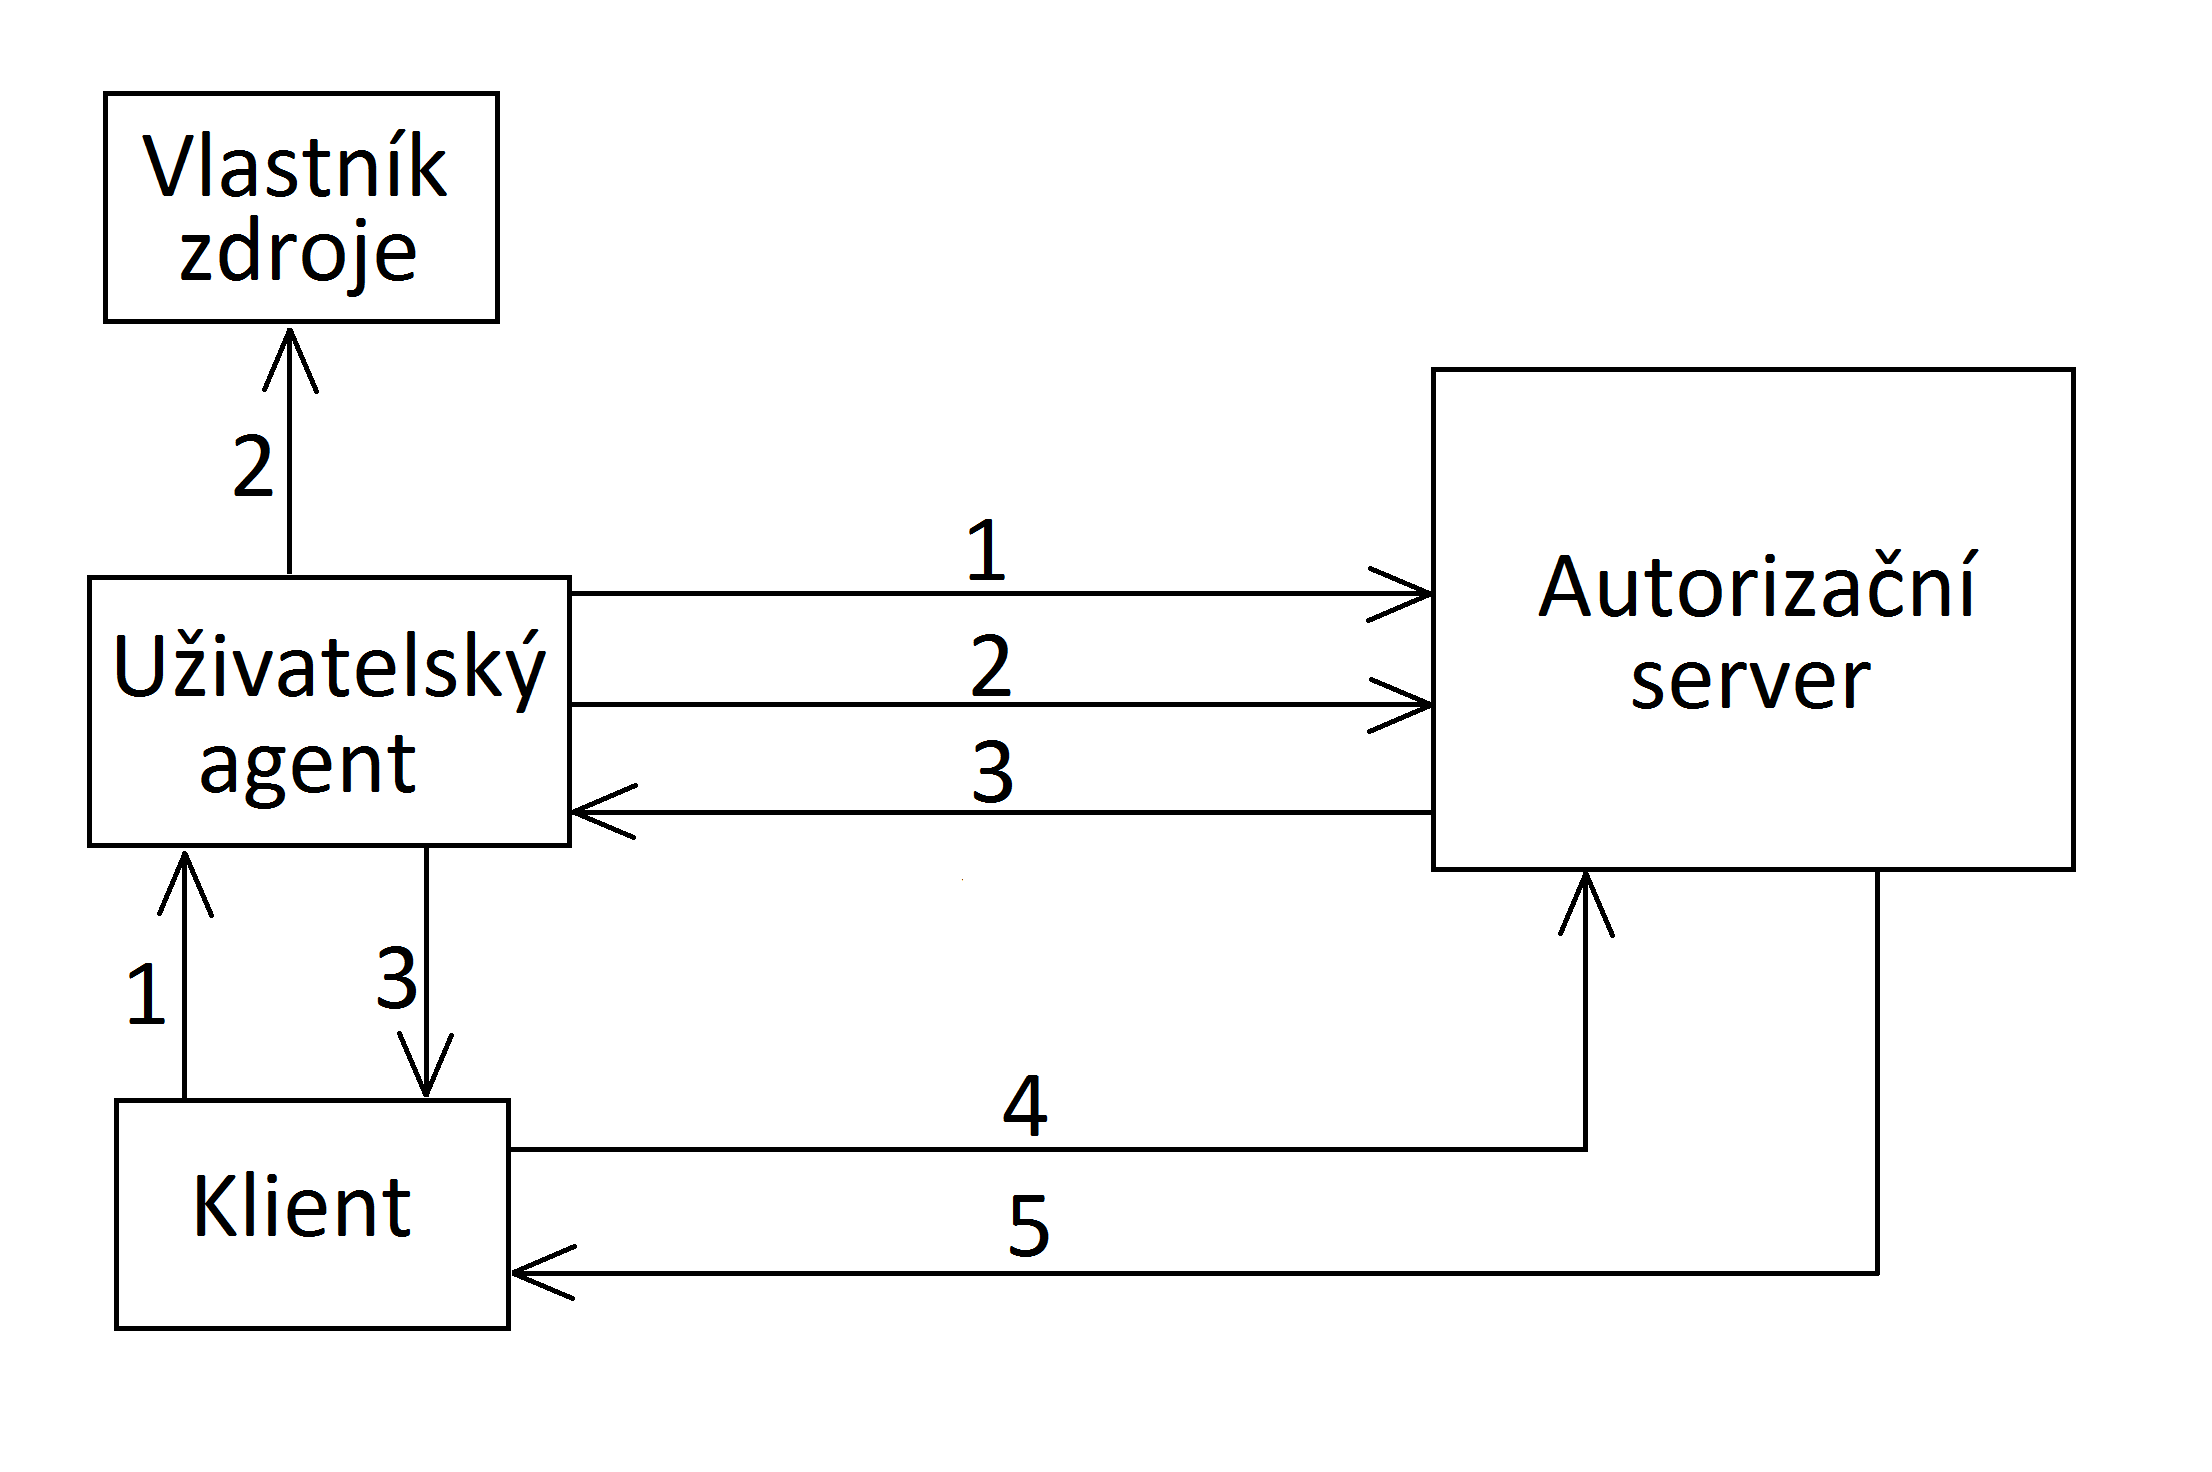
\includegraphics[width=\textwidth]{/home/oprikryl/Skola/bakalarka/obrazky/oauth.png}
  		\end{minipage}
		\end{center}
 		\caption{OAuth 2.0 - Autorizace autorizačním kódem.}
  		\label{fig:oauth}
	\end{figure}

	\begin{enumerate}
		\item {
		Klient pomocí prohlížeče přesměruje vlastníka zdroje na autorizační server. Klient v 				požadavku uvede svůj identifikátor, požadovaný rozsah přístupu,  identifikační řetězec
			\footnote {
			Identifikační řetězec (tzv. state) slouží k identifikaci sezení při větším počtu různých 				OAuth požadavků.
			}	 
		a adresu, na kterou má být zaslán autorizační kód.
		}
		\item
		Vlastník zdroje se autentizuje serveru a potvrdí klientovi přístup o daném rozsahu.
		\item
		Autorizační server přesměruje prohlížeč na adresu obdrženou v\,prvním kroku a předá jí 			autorizační kód a identifikační řetězec obdržený v prvním kroku.
		\item
		Klient zažádá autorizační server o přístupový token. V požadavku uvede autorizační kód 			přijatý v předchozím kroku, identifikátor klienta, příslušné heslo a adresu použitou k 				získání autorizačního kódu v prvním kroku. 
		\item	
		Autorizační server zkontroluje identifikační údaje klienta a ověří platnost autorizačního 				kódu. Jestliže jsou všechny údaje platné, autorizační server zašle přístupový a obnovující 			token klientovi.

	\end{enumerate}

	\section{Úpravy systému RemSig}

	RemSig v nynější podobě rozeznává dvě základní role. Role \textit{Signer} je určena pouze pro 		podepisování dat, zatímco role \textit{Manager} pouze pro správu systému. Implementace 			knihoven však využívá funkcionalitu obou rolí. Z tohoto důvodu bude vytvořena nová role, 			která bude obsahovat následující funkce:
	\begin{itemize}
		\item \textit{listMyCertificates} - vypíše certifikáty přihlášeného uživatele

		\item \textit{checkPassword} - zkontroluje heslo k privátnímu klíči

		\item \textit{sign} - vytvoří digitální podpis
	\end{itemize}

	Nová role bude určena přímo pro knihovny integrující RemSig do klientských aplikací. Jelikož 		je jako autentizační metoda těchto knihoven použit protokol OAuth a pro server je možné 			získat z přístupového tokenu identitu uživatele, všem výše uvedeným metodám je odebrán 		parametr \textit{"uco"}, který sloužil k identifikaci uživatele.

	\section{PKCS\#11 modul}
	
	V druhé části praktické práce jsem implementovat PKCS\#11 modul, který slouží k propojení 		systému RemSig a aplikací, které modul PKCS\#11 podporují. Mezi tyto aplikace patří například 	Mozilla Firefox, Safari, Mozilla Thunderbird, Evolution a mnoho dalších
\footnote{Seznam podporovaných aplikací: \url{https://github.com/OpenSC/OpenSC/wiki/Using-smart-cards-with-applications}.}. 
	Standard PKCS\#11 nepředpisuje, aby všechny jeho funkce byly implementovány, avšak 			definuje, které funkce by měli být implementovány, aby modul poskytoval nějakou funkcionalitu. S ohledem 	na systém RemSig byl vytvořen profil PKCS\#11, který umožňuje práci s digitálním podpisem. 		Virtuální zařízení - token, je zobrazováno jako zařízení pouze pro čtení a tím pádem všechny 		funkce, které vytvářejí, upravují nebo mažou objekty, nejsou podporovány. Každý aktivní token je 	již inicializován a uživatel má nastavené přihlašovací heslo. Aktivní token zároveň obsahuje 			právě jeden certifikát a jeden soukromý klíč.

	\subsection{Obecné funkce} 
	\textit{C\_Initialize} - inicializuje celý modul a vytvoří kontext klientské strany, který slouží k 		uchovávání informací o modulu. Tato funkce dále nastavuje logování a získává certifikáty z 			úložiště RemSig. Ke každému certifikátu obdrženému metodou \textit{listMyCertificates} je 			vytvořen virtuální token, který je posléze připojen do virtuálního slotu. 
	\newline
 	\newline
	\textit{C\_Finalize} - tato funkce je volána při ukončení práce s modulem. Slouží k uvolnění 			kontextu a k uzavření souboru logování.
	\newline
	\newline
	\textit{C\_GetFunctionList} - obsahuje seznam všech implementovaných funkcí modulu.
	\newline
	\newline
	\textit{C\_GetInfo} - poskytuje informace o modulu. Je zde uvedena použitá verze 				cryptoki a název, výrobce a verze modulu.

	\subsection{Správa modulu} 

	\textit{C\_GetSlotList} - slouží k získání seznamu dostupných slotů. Aplikace může 				určit, zda-li má být navrácen kompletní seznam nebo pouze seznam slotů, ve kterých je 			přítomen token.
	\newline
	\newline
	\textit{C\_GetSlotInfo} - představuje základní informace o každém statickém slotu.
	\newline
	\newline
	\textit{C\_GetTokenInfo} - slouží k získání informací o tokenu. Funkce nastaví tokenu 				hodnoty popis, sériové číslo a vydavatel podle certifikátu, který obsahuje. Dále každému 			tokenu nastaví následující vlastnosti:
		\begin{itemize}
		\item \textit{CKF\_WRITE\_PROTECTED} - token je pouze pro čtení.

		\item \textit{CFK\_LOGIN\_REQUIRED} - uživatel musí být přihlášen pro přístup k 				některým objektům a funkcím.

		\item \textit{CKF\_USER\_PIN\_INITIALIZED} - PIN uživatele je již nastaven, zabrání 				volání funkce \textit{C\_InitPin}.

		\item \textit{CKF\_TOKEN\_INITIALIZED} - token je již inicializován, zabrání volání funkce 			\textit{C\_InitToken}.
		\end{itemize}
	\textit{C\_GetMechanismList} - funkce vrací seznam podporovaných kryptografických 				mechanismů tokenu. V seznamu se nyní nachází pouze jeden prvek a to 							\textit{CKM\_SHA256\_RSA\_PKCS}, který odpovídá základnímu mechanismu metody 			\textit{sign} používané systémem RemSig.
	\newline
	\newline
	\textit{C\_GetMechanismInfo} - slouží k získání podrobných informací o mechanismu.

	\subsection{Správa relací} 

	\textit{C\_OpenSession} - vytvoří novou relaci mezi aplikací a tokenem. Jestliže má token již 		otevřenou existující relaci s aplikací, synchronizuje jejich stavy.
	\newline
	\newline
	\textit{C\_CloseSession} - uzavře relaci a uvolní paměť.
	\newline
	\newline
	\textit{C\_CloseAllSessions} - ukončí všechny relace a uvolní paměť, je volána před ukončením 	práce s modulem.
	\newline
	\newline
	\textit{C\_GetSessionInfo} - poskytuje informace o relaci, její stav, ID slotu, ke kterému je 			vytvořena a další.
	\newline
	\newline
	\textit{C\_Login} - autentizuje uživatele tokenu. Při úspěšném přihlášení, funkce nastaví 			uživateli příslušnou roli, čímž uživatel získá přístup k privátním objektům a funkcím. Všechny 		relace, které souvisí se stejným tokenem, jsou následně aktualizovány do přihlášeného stavu. 		PIN je uložen do kontextu tokenu.
	\newline
	\newline
	\textit{C\_Logout} - odhlásí uživatele a uvolní paměť. Všechny relace jsou aktualizovány do 		nepřihlášeného stavu.

	\subsection{Práce s objekty a digitální podpis}

	\textit{C\_FindObjectsInit} - inicializuje vyhledávání objektů, poskytnutá šablona je uložena do 	kontextu relace, která použila funkci.
	\newline
	\newline
	\textit{C\_FindObjects} - zahájí samotné vyhledávání objektů. Každý token vlastní jeden 			certifikát a k němu jeden privátní klíč. Jestliže je objekt nalezen, funkce vrací identifikátor 			objektu.
	\newline
	\newline
	\textit{C\_FindObjectsFinal} - ukončí operaci vyhledávání a uvolní šablonu z\,relačního 				kontextu.
	\newline
	\newline
	\textit{C\_GetAttributeValue} - funkce slouží k získání atributu objektu, opět je poskytnuta 			šablona, která určuje, které atributy jsou požadovány. 
	\newline
	\newline
	\textit{C\_SignInit} - inicializuje proces digitálního podpisu dat. Funkci je předán soukromý klíč a 		mechanismus, který bude použit při digitálním podpisu.
	\newline
	\newline
	\textit{C\_Sign} - funkce provede digitální podpis dat pomocí metody \textit{sign} systému 			RemSig.

	\subsection{Práce s modulem}
	
	Jestliže chce aplikace pracovat s modulem, pak musí pro jeho plnou funkčnost splnit sérii 			příkazů. Typickým příkladem práce aplikace s\,modulem je následující posloupnost:
	\begin{enumerate}
		\item Uživatel musí získat přístupový token pomocí OAuth aplikace. Jestliže token není k 			dispozici, modul se nepodaří inicializovat.
		\item Aplikace inicializuje modul, který získá certifikáty ze systému RemSig.
		\item Poté si aplikace vylistuje dostupné tokeny a vybere si token, se kterým chce 				pracovat. Aplikace si může získat informace o\,tokenu a mechanismech, které podporuje.
		\item Pro práci s tokenem si aplikace vytvoří jednu nebo více relací pomocí funkce 					\textit{C\_OpenSession}.
		\item V tomto stavu je možné vyhledat veřejné objekty tokenu. Pro přístup k privátním 			objektům je zapotřebí se přihlásit pomocí funkce \textit{C\_Login}. PIN k tokenu je 				odeslán systému RemSig pro ověření správnosti. Po úspěšném přihlášení jsou 					aktualizovány všechny relace do přihlášeného stavu.
		\item Aplikace inicializuje vyhledávání objektů pomocí funkce \textit{C\_Find}- \textit{ObjectsInit}, 			přičemž funkci předá šablonu, která specifikuje hledaný objekt. 
		\item Následuje samotné vyhledávání objektů. Funkce \textit{C\_FindObjects} získá 				identifikátory objektů, které se shodují s parametry šablony.
		\item Vyhledávání je ukončeno zavoláním funkce \textit{C\_FindObjectsFinal}, paměť 				obsahující šablonu je uvolněna.
		\item Aplikace vykoná kryptografické operace, v našem případě digitální podpis dat. Pro 			použití jiného tokenu není potřeba opět inicializovat modul, ale lze začít od kroku číslo 				3.
		\item Při ukončení práce s modulem jsou zavolány funkce \textit{C\_Close}- \textit{Sessions} nebo 		\textit{C\_CloseAllSessions}, které ukončí relace mezi aplikací a tokenem a následně 				\textit{C\_Finalize}, který uvolní kontext modulu.
	\end{enumerate}

	\section{Smard card minidriver}
	Ve třetí části praktické práce jsem implementoval Smart card minidriver, který slouží k propojení 	systému RemSig a úložiště certifikátů operačního systému Windows. Vytvořený minidriver 			podporuje načtení jak pod Smart Card BaseCSP, tak i pod CNG Key Service Provider. Každý 		certifikát v systému RemSig je zobrazován jako samostatný token, který má vlastnost pouze 		pro čtení. Dokumentace minidriveru přesně specifikuje, které funkce musí být implementovány, 		jestliže je token pouze pro čtení.

		\subsection{Obecné funkce}
		\textit{CardAcquireContext} - inicializuje komunikaci mezi BaseCSP/KSP a minidriverem. 			BaseCSP/KSP předá minidriveru strukturu obsahující informace o kartě (jméno, ATR), o 				požadované verzi knihovny a\,o\,funkcích, které slouží pro práci s daty (alokace paměti, 			uvolnění paměti, cache). Jestliže je karta minidriverem rozpoznána, funkce vytvoří 				kontext karty a pomocí metody \textit{listMyCertificates} získá certifikát ze systému 				RemSig a uloží si jej do kontextu. Nakonec funkce přidá do struktury tabulku funkcí, 			které minidriver implementuje. Minimální podporovaná verze minidriveru je verze 4.
		\newline
 		\newline
		\textit{CardQueryCapabilities} - získá přehled možností karty. V aktuální verzi jsou 				definovány pouze 2 vlastnosti - možnost karty generovat klíče, kterou karta pouze pro 			čtení nedisponuje, a zda-li karta provádí vlastní kompresi dat (není nutná komprese v 				baseCSP/KSP). Nastavením této hodnoty na pravda zamezíme kompresi souborů zvenčí.
		\newline
 		\newline
		\textit{CardGetProperty} - slouží k získání vlastností karty. Touto operací lze získat 				vlastnosti, jako jsou například sériové číslo karty, podporované kryptografické mechanismy 			a informaci, zda je karta pouze pro čtení.
		\newline
 		\newline
		\textit{CardDeleteContext} - tato funkce je volána při ukončení práce s minidriverem. 				Slouží k uvolnění veškerého kontextu, který minidriver alokoval.

		\subsection{Přihlášení a odhlášení}
		\textit{CardAuthenticatePin} - autentizuje uživatele tokenu. Heslo k tokenu je 					zkontrolováno pomocí metody \textit{checkPassword}. Při úspěšném přihlášení, funkce 			nastaví uživateli příslušnou roli, čímž uživatel získá přístup k privátním objektům a funkcím.
		\newline
 		\newline
		\textit{CardDeauthenticate} - odhlásí uživatele a uvolní paměť. Tato funkce je definována 			jako volitelná.
		\newline
		\newline
		\textit{CardAuthenticateEx} - tato funkce nahrazuje funkci \textit{CardAuthenticatePin}, 			která je určena pro nižší verze. Tato funkce kromě klasického přihlášení heslem přidává 			podporu externí autentizace (např. pomocí biometriky), autentizace typu výzva/odpověď a 			další. Implementace minidriveru podporuje pouze klasické přihlášení pomocí hesla. Heslo k 			tokenu je opět zkontrolováno pomocí metody \textit{checkPassword}. Při úspěšném 				přihlášení, funkce nastaví uživateli příslušnou roli, čímž uživatel získá přístup k privátním 			objektům a funkcím.
		\newline
 		\newline
		\textit{CardDeauthenticateEx} - tato funkce nahrazuje funkci \textit{CardDeauthenticate}, 		která je určena pro nižší verze. Funkce odhlásí uživatele a uvolní paměť. Jestliže funkce není 				dostupná a je vyžadováno odhlášení, systém se pokusí restartovat kartu.
		
		\subsection{Operace s veřejnými daty}
		Jelikož minidriver pracuje s virtuálním tokenem, je zapotřebí virtualizovat souborový 				systém. V implementaci jsou zahrnuty všechny podstatné soubory pro správný chod 				minidriveru dle jeho specifikace.
		\newline
		\newline
		\textit{CardEnumFiles} - slouží k získání řetězce souborů ve složce určené parametrem.
		\newline
 		\newline
		\textit{CardReadFile} - získá obsah požadovaného souboru.
		\newline
		\newline
		\textit{CardGetFileInfo} - získá informace o velikosti a přístupových právech souboru.
		\newline
 		\newline
		\textit{CardQueryFreeSpace} - funkce indikuje, kolik je na kartě kontejnerů, určuje 				maximální počet kontejnerů a velikost volného místa. Jelikož je karta pouze pro čtení, k 			dispozici není žádné volné místo a aktuální i\,maximální počet kontejnerů je 1.

		\subsection{Kontejnery}
		\textit{CardGetContainerInfo} - slouží k obdržení veřejného klíče. Klíč musí být 			ve formátu DER.
		\newline
 		\newline
		\textit{CardGetContainerProperty} - získá vlastnosti kontejneru, jedná se o alternativní 			funkci k \textit{CardGetContainerInfo}.
		\newline
		\newline
		\textit{CardQueryKeySizes} - vrací délku veřejných klíčů, které jsou podporované 				zařízením.

		\subsection{Kryptografické operace}
		\textit{CardSignData} - provede digitální podpis dat pomocí metody  \textit{sign} systému 			RemSig. 

	\section{Virtualizace zařízení v operačním systému Windows}
	
	Proces objevení karty je nedílnou součástí práce s kryptografickými zařízeními v operačním 			systému Windows, který nenabízí tak vysokou úroveň abstrakce jako PKCS\#11 modul. Na 		samém dnu modelu se nachází knihovna \textit{Winscard.dll}, která slouží k přiřazení karty k\,odpovídajícímu minidriveru. Po připojení karty je získán jednoznačný identifikátor karty (nazýván 		ATR), který se operační systém pokusí vyhledat v systémovém registru, v němž jsou uloženy 		záznamy o kryptografických zařízeních, jejich identifikátorech a příslušných cestách\,k 				odpovídajícím minidriverům.

	Jelikož se v návrhu žádné fyzické zařízení nevyskytuje, je zapotřebí vytvořit ovladač k virtuální 		čtečce karet a simulovat vložení karty do systému, což vyvolá signál ke spuštění minidriveru. Při 	hledání této problematiky jsem našel spoustu komerčních modelů, které využívají výše 			popsaný princip simulace vložení karty, ovšem žádný volně šířitelný aktuální model. Díky 			nemožnosti virtualizace karty nebyl implementovaný minidriver nijak testován a jedná se pouze 		o\,prototyp.

	\section{Budoucí rozšíření knihoven a poznámky k systému RemSig}
	Knihovny nyní podporují jen základní metodu pro podpis dat systémem RemSig. Tato metoda 		vytvoří haš dat za využití hašovací funkce SHA256 a ten posléze zašifruje soukromým klíčem 		pomocí algoritmu RSA. Do knihoven by bylo možné přidat podporu PKCS\#7 profilů, které 			systém RemSig podporuje metodou \textit{signPKCS7}.  \newline

	Bezpečnostní token je zařízení, které může vlastnit více certifikátů a privátních klíčů, které jsou 		chráněné jedním společným heslem (heslem zařízení). Současná implementace systému RemSig 		však přiřazuje každému privátnímu klíči samostatné heslo, čímž úložiště představuje \textit{n} 		tokenů pro \textit{n} dvojic privátních klíčů a certifikátů. Vzhledem k\,velkému počtu certifikátů v 	úložišti by mohli být certifikáty rozděleny do několika skupin (např. komerční, atd...), které by 		byly chráněny jednotným heslem. Tímto by se rapidně snížil počet virtuálních tokenů 				simulovaných v knihovně PKCS\#11 a virtualizovaných pro minidriver.
	
	\section{Externí závislosti}

		\subsection {Libcurl} 
		Libcurl je multiplatformní klientská knihovna sloužící k přenosu dat, jejíž výhody jsou 				například jednoduchost použití, množství podporovaných protokolů a možnost použití 				zdarma.  Mezi podporované protokoly patří FTP, HTTP, HTTPS, LDAP a mnohé další. 				Podporované platformy zahrnují mezi jinými také Solaris, NetBSD, Mac OS X a Linux. 				Klíčovými vlastnostmi knihovny, které ji činí jednoduchou k\,použití, je podpora vícevláken, 			IPv6 a důkladná dokumentace.

		\subsection {OpenSSL} 
		OpenSSL je multiplatformní open source projekt, který poskytuje knihovny implementující základní 				kryptografické funkce. Projekt je napsán v jazyce C, ale poskytuje mnoho tzv. "wrapperů", 			díky kterým je možné knihovny používat i v ostatních programovacích jazycích. Aktuální 			verze je 1.0.2 vydána k 22. lednu 2015, ale v průběhu tohoto roku je očekávána nová 			implementace s označením 1.1.0.

		\subsection {Libxml2} 
		Libxml2 je nástroj vyvinutý pro platformu Gnome, sloužící k práci s XML soubory. Navzdory 		původu v Gnome je použitelný i na jiných platformách včetně Windows a MacOS. Co si z 				Gnome zachovává je použitelnost zdarma, obsáhlá dokumentace, široká podpora a 				uživatelská základna a v neposlední řadě kompatibilita s mnoha programovacími jazyky.

\let\cleardoublepage\clearpage

\chapter{Závěr}

Cílem bakalářské práce bylo popsat systém RemSig a představit moduly, které slouží k integraci jeho funkcionality do klientských aplikací. V práci je detailně popsán standard PKCS\#11, kryptografické prostředí operačního systému Microsoft Windows a protokol OAuth 2.0. Výsledkem bakalářské práce jsou knihovny propojující systém RemSig a klientské aplikace. Ačkoliv se v průběhu implementace vyskytlo několik překážek, modul PKCS\#11 a Smart Card Minidriver byly úspěšně vytvořeny. Díky jejich implementaci již není zapotřebí používat webové rozhraní INET a IS MU, což zaměstnancům MU výrazně usnadní práci při podepisování digitálních dokumentů. Nezávislost systému na webovém rozhraní univerzity také umožňuje jeho rozšíření mimo univerzitní kruhy.

\chapter{Bibliografie}
{\flushleft
\begin{itemize}
	
	\item[$\mbox{[1]}$] Katz, J. \textit{Digital Signatures}. New York: Springer US, 2010, 192 p. ISBN 0387277110.

	\item[$\mbox{[2]}$] Vigašová, S. \textit{Client Tools for RemSig} [online]. Brno: Masarykova univerzita, 2015 [cit. 20. 5. 2016]. 48 s. Dostupné na: \url{https://is.muni.cz/auth/th/409781/fi_b/vigasova_bp.pdf}

	\item[$\mbox{[3]}$] Hardt, D. \textit{The OAuth 2.0 Authorization Framework} [online]. Internet Engineering Task Force, 2012[cit. 20. 5. 2016]. 76 s. Dostupné na: \url{http://tools.ietf.org/html/rfc6749}

	\item[$\mbox{[4]}$] Jirůtka, J. \textit{OAuth 2.0} [online]. Praha: Wiki FIT ČVUT, 26. 2. 2014, [akt. 30. 3. 2016], [cit. 20. 5. 2016].  Dostupné na: \url{https://rozvoj.fit.cvut.cz/Main/oauth2}

	\item[$\mbox{[5]}$] \textit{PKCS \#11 v2.20: Cryptographic Token Interface Standard} [online]. RSA Laboratories, 2004 [cit. 20. 5. 2016]. 407 s. Dostupné na: \url{ftp://ftp.rsasecurity.com/pub/pkcs/pkcs-11/v2-20/pkcs-11v2-20.pdf}

	\item[$\mbox{[6]}$] Kubina, T. \textit{Vzdialené PKCS\#11 úložisko} [online]. Brno: Masarykova univerzita, 2010 [cit. 20. 5. 2016]. 56 s. Dostupné na: \url{https://is.muni.cz/auth/th/172593/fi_m/dp.pdf}

	\item[$\mbox{[7]}$] Scholz, F. \textit{PKCS11 Implement} [online]. Mozilla Developer Network and individual contributors, 13. 7. 2007, [akt. 7. 5. 2014], [cit. 20. 5. 2016]. Dostupné na: \url{https://developer.mozilla.org/en-US/docs/Mozilla/Projects/NSS/PKCS11_Implement}

	\item[$\mbox{[8]}$]Tarasov, V., Rousseau, L. \textit{OpenSC – tools and libraries for smart cards} [online]. GitHub, 11. 12. 2012, [akt. 15. 1. 2016], [cit. 20. 5. 2016]. Dostupné na: \url{https://github.com/OpenSC/OpenSC/wiki}

	\item[$\mbox{[9]}$] Coleridge, R. \textit{The Cryptography API, or How to Keep a Secret} [online]. Microsoft Developer Network Technology Group, 19. 8. 1996, [cit. 20. 5. 2016]. Dostupné na: \url{https://msdn.microsoft.com/en-us/library/ms867086.aspx}

	\item[$\mbox{[10]}$] \textit{Cryptography API: Next Generation} [online]. Microsoft Developer Network, [cit. 20. 5. 2016]. Dostupné na: \url{https://msdn.microsoft.com/en-us/library/windows/desktop/aa376210(v=vs.85).aspx}

	\item[$\mbox{[11]}$] \textit{CryptoAPI Cryptographic Service Providers} [online]. Microsoft Developer Network, [cit. 20. 5. 2016]. Dostupné na: \url{https://msdn.microsoft.com/en-us/library/windows/desktop/bb931357(v=vs.85).aspx}

	\item[$\mbox{[12]}$] Mysore, S. \textit{Smart Card Base Cryptographic Service Provider (Base CSP)} [online]. Microsoft Developer Network Blog, 30. 11. 2005, [cit. 20. 5. 2016]. Dostupné na: \url{https://blogs.msdn.microsoft.com/shivaram/2005/11/30/smart-card-base-cryptographic-service-provider-base-csp/}

	\item[$\mbox{[13]}$] \textit{Windows Smart Card Minidriver Specification} [online]. Microsoft Developer Network, 9. 7. 2009, [akt. 25. 2. 2016], [cit. 20. 5. 2016]. Dostupné na: \url{http://download.microsoft.com/download/3/3/2/332FD70B-F04D-470A-A135-040350B9563F/sc-minidriver_specs_v7.07.docx}
\end{itemize}
}


\appendix %% Start the appendices.
\chapter{Přílohy}

	\begin{itemize}
		\item bp.pdf - elektronická verze práce ve formátu pdf

		\item oauth - složka obsahující zdrojové kódy protokolu OAuth 2.0 a spustitelné binárky

		\item pkcs11 - složka obsahující implementaci PKCS\#11 modulu, testovacího souboru a  			knihovny ve formě \textit{.so} souboru

		\item minidriver - složka obsahující implementaci Smart Card Minidriveru
	\end{itemize}

\chapter{Použití PKCS\#11 modulu}
	OAuth 2.0: \newline
	Před načtením PKCS\#11 modulu je zapotřebí získat přístupový token k systému Remsig. Aplikace OAuth vytvoří složku, do které po úspěšné autentizaci uloží tyto přistopové údaje. Jestliže není soubor, či složka k dispozici, anebo není přístupový token platný, PKCS\#11 modul se nepodaří načíst.
	\newline
	\newline
	Přidání PKCS\#11 modulu do poštovního klienta Mozilla ThunderBird:
	\begin{enumerate}
		\item Uložte si PKCS\#11 modul na permanentní místo na lokálním disku.
		\item Po spuštění klienta otevřete okno nastavení. Zvolte "Zabezpečení", dále 					"Bezpečnostní zařízení".
		\item Ve správci bezpečnostních zařízení zvolte možnost "Načíst".
		\item Nyní pomocí možnosti "Procházet" zvolte cestu k \textit{.so} souboru modulu a 				potvrďte tlačítkem "Ok".
	\end{enumerate}
	
		\begin{figure}[!ht]
  			\begin{minipage}{1.00\textwidth}
    				\includegraphics[width=\textwidth]{/home/oprikryl/Skola/bakalarka/obrazky/Appendix_pkcs11install2.png}
  			\end{minipage}
 			\caption{RemSig PKCS11 modul.}
  			\label{fig:RemSig PKCS11 modul.}
		\end{figure}	
	
\end{document}